\section{Measurement}
\begin{outline}

\0
\subsection{Length reiterated}
	\1 Perimeter of polygons
		\2 The perimeter of a polygon is the sum of the length of its sides, essentially being the distance around the outside of the polygon. For a simple application such as a quadrilateral, the perimeter can be found by adding together all four side lengths. When in special circumstances, such as working with a square, where all sides are equal, multiplication can be used instead of addition as a way of simplifying the equation.
			\3 Perimeter of a rectangle
				\[P = 2l + 2w = 2(l + w)\]
			\3 Perimeter of a square
				\[P = 4l\]
			\3 Perimeter of a triangle
				\[P = a + b + c\]
	\1 Circumference of a circle
		\2 The circumference (equivalent to a perimeter, but a circle has no sides) of a circle is the distance around the outside of a circle. It is found by multiplying twice the radius of the circle (essentially the diameter) with $\pi$. This is the case because of the relationship between the diameter and the circumference, where the circumference is always $\pi$ times the diameter.
			\3 There are two equations generally used to find the circumference of a circle. They are applied depending on what information is given.
				\[C = 2\pi r = \pi d\]
	\1 Perimeter of a sector
		\2 A sector is a portion of a circle, much like a slice out of a pie.
			\3 The equation to find the perimeter of a sector uses the greek letter theta, represented as $\theta$, to identify the variable angle of the sector.
				\[P = 2r+ \frac{\theta}{360} \times 2\pi r\]

\0
\subsection{Pythagoras' theorem}
	\1 Why it is used
		\2 Pythagoras' theorem is applicable only to right-angled triangles. The Pythagoras' theorem is used when one has the length of two sides of a triangle, and wants to find the third.
\begin{center}
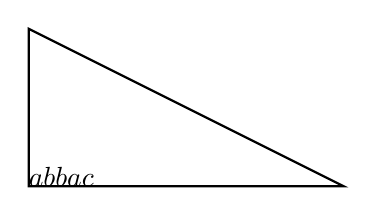
\begin{tikzpicture}[thick]
\coordinate (O) at (0,0);
\coordinate (A) at (4,0);
\coordinate (B) at (0,2);
\draw (O)--(A)--(B)--cycle;

\tkzLabelSegment[below=2pt](O,A){\textit{$a$ or $b$}}
\tkzLabelSegment[left=2pt](O,B){\textit{$b$ or $a$}}
\tkzLabelSegment[above right=2pt](A,B){\textit{$c$}}

\tkzMarkRightAngle[fill=white,size=0.5,opacity=.4](A,O,B)
\tkzLabelAngle[pos = 0.35](A,O,B){}

\end{tikzpicture}
\end{center}
	\1 Finding each side of the right-angled triangle
		\2 The longest side of the right-angled triangle is called the hypothesis. Coincidentally, the most common form of Pythagoras' theorem is for finding the hypothesis. Pythagoras' theorem can be used to find any side of a triangle, assuming one has the other two side lengths. The theorem must, however, be rearranged in order to find the other sides. For demonstrations of the Pythagoras theorem, often the letters $a$, $b$, and $c$ are used. $a$ and $b$ can be used at will, but $c$ is generally accepted to be the hypothesis.
			\3 Finding the hypothesis
				\[a^2 + b^2 = c^2\]
				\[\sqrt{a^2 + b^2} = c\]
			\3 Finding other sides
				\[c^2 - b^2 = a^2\]
				\[c^2 - a^2 = b^2\]
				\[\sqrt{c^2 - b^2} = a\]
				\[\sqrt{c^2 - a^2} = b\]

\0
\subsection{Area}
	\1 What is area?
		\2 Area is a measure of surface. As such, area is always expressed as square units, such as cm$^2$ and m$^2$. For example, a rectangle with 5 metres of width and 10 metres of length would have 50 metres squared of area.
	\1 Equations to find area
		\2 Area is usually found using a simple equation, but more complex shapes (called composite shapes) or a polygon can be separated into a number of simple equations that can be added together to find the area.
			\3 Area of a square
				\[A = l^2\]
			\3 Area of a rectangle
				\[A = lw\]
			\3 Area of a triangle
				\[A = \frac{1}{2}bh\]
			\3 Area of a rhombus/kite
				\[A = \frac{1}{2}xy\]
			\3 Area of a parallelogram
				\[A = bh\]
			\3 Area of a trapezium
				\[A = \frac{1}{2}(a+b)h\]
			\3 Area of a circle
				\[A = \pi r^2\]
			\3 Area of a sector
				\[A = \frac{\theta}{360}\pi r^2\]
	\1 Converting between units of area
		\2 To convert between units of area, one must realise that area is a squared unit, hence it is necessary to convert by $\times x^2$ or $\div x^2$ (where $x$ is 10, 100, 1000, etc.) instead of $\times x$ or $\div x$.
	\1 Using area to find unknown lengths
		\2 As the area of a polygon can be found with an equation, the equation can be rearranged to find side lengths. For example, knowing that $A = l^2$ is the equation for the area of a square, the reverse of the square operation, the square root, can be used to find the length from the area. The rearrangement of the equation would be $l = \sqrt{A}$, and is a perfectly acceptable way of finding the length of the sides within a square.

\0
\subsection{Surface area -- prisms and cylinders}
	\1 Finding the surface area of a prism
		\2 The surface area of a prism is found by adding the area of each face of the prism. In the case of, for instance, a triangular prism, there are two end faces, and the three faces created by the extrusion of the triangle.
	\1 Finding the surface area of a cylinder
		\2 The surface area of a cylinder is found by adding the area of the two circular ends to the area created by the circumference of the circles multiplied by the height of the cylinder.
			\3 Surface area of a cylinder
				\[SA = 2\pi r^2 + 2\pi rh\]

\0
\subsection{Surface area -- pyramids and cones}
	\1 Finding the surface area of a pyramid
		\2 The surface area of a pyramid is found by adding the base area of the pyramid to the area of the four triangles.
			\3 Surface area of a pyramid
				\[l^2 + 4 \times \frac{1}{2}bh\]
	\1 Finding the surface area of a cone
		\2 A cone is composed of a circle as the base, and a sector. The surface area of a cone is found by multiplying $\pi$, the radius and the slant length, then adding the area of the base.
			\3 Surface area of a cone
				\[\pi rs + \pi r^2\]

\0
\subsection{Volume -- prisms and cylinders}
	\1 Finding the volume of a prism
		\2 A prism is a polygon extended along the height axis, and as such has a uniform cross-section. The prism is named by the shape of the cross-section, hence ``triangular prism'', ``hexagonal prism'', etc. The volume of a prism is found by multiplying the area of the cross-section by the height. Thus, the formula for the volume of a prism is always the same, regardless of the cross-sectional shape.
			\3 Volume of a prism
				\[V = ah\]
	\1 Finding the volume of a cylinder
		\2 A cylinder is a circle extended along the height axis, and because of that has a perfect circle as the cross-section. The equation used to find the volume of the cylinder is the area of the circle multiplied by the height of the cylinder.
			\3 Volume of a cylinder
				\[V = ah = \pi r^2 h\]

\0
\subsection{Volume -- pyramids and cones}
	\1 Finding the volume of a pyramid
		\2 A pyramid within a cube takes up one third of the space. Therefore, the volume of a pyramid is the area of the base multiplied by the height, divided by 3.
			\3 Volume of a pyramid
				\[V = \frac{1}{3}ah\]
	\1 Finding the volume of a cone
		\2 A cone within a cube takes up one third of the space. Hence, the volume of the cone is the area of the base multiplied by the height, divided by 3.
			\3 Volume of a cone
				\[V = \frac{1}{3}ah\]

\0
\subsection{Spheres}
	\1 Finding the volume of a sphere
		\2 The volume of a sphere is calculated by multiplying the equation 4/3 by $\pi r^3$.
			\3 Volume of a sphere
				\[V = \frac{4}{3}\pi r^3\]
	\1 Finding the surface area of a sphere
		\2 The surface area of a sphere is calculated by multiplying 4 by $\pi r^2$.
			\3 Surface area of a sphere
				\[SA = 4\pi r^2\]
	\1 Finding the radius of a sphere
		\2 The radius of a sphere can be found using the volume of the sphere. Knowing the equation for volume of a sphere allows one to substitute in the known volume and solve the problem like a regular equation.

\end{outline}
